%-----------------------------------------------------------------------------------------------------------------
%   Submission Information
%-----------------------------------------------------------------------------------------------------------------
%  Article submitted by: Assoc. Prof. Dr. Yasemin P. Kahya
%  Journal submitted to: Physiological Measurement
%  Article title: A DSP based instrument for real-time classification of pulmonary sounds
%  Authors: Sameer Alsmadi and Yasemin P. Kahya
%  Article type: Paper
%  Postal address: Electrical and Electronics Engineering Department
%		  Bogazici University
%		  Bebek Istanbul 34342
%		  Turkey
%  E-mail address: kahya@boun.edu.tr 
%  Phone number: (+90) 212 358 15 40/1851
%  Fax number: (+90) 212 287 24 65
%-----------------------------------------------------------------------------------------------------------------



%%%%%%%%%%%%%%%%%%%%%%%%%%%%%%%%%%%%%%%%%%%%%%%%%%%%%%%%%%%%%%%%%%%%%%%%
%    INSTITUTE OF PHYSICS PUBLISHING                                   %
%                                                                      %
%   `Preparing an article for publication in an Institute of Physics   %
%    Publishing journal using LaTeX'                                   %
%                                                                      %
%    LaTeX source code `ioplau2e.tex' used to generate `author         %
%    guidelines', the documentation explaining and demonstrating use   %
%    of the Institute of Physics Publishing LaTeX preprint files       %
%    `iopart.cls, iopart12.clo and iopart10.clo'.                      %
%                                                                      %
%    `ioplau2e.tex' itself uses LaTeX with `iopart.cls'                %
%                                                                      %
%%%%%%%%%%%%%%%%%%%%%%%%%%%%%%%%%%%%%%%%%%%%%%%%%%%%%%%%%%%%%%%%%%%%%%%%
%
%
% First we have a character check
%
% ! exclamation mark    " double quote  
% # hash                ` opening quote (grave)
% & ampersand           ' closing quote (acute)
% $ dollar              % percent       
% ( open parenthesis    ) close paren.  
% - hyphen              = equals sign
% | vertical bar        ~ tilde         
% @ at sign             _ underscore
% { open curly brace    } close curly   
% [ open square         ] close square bracket
% + plus sign           ; semi-colon    
% * asterisk            : colon
% < open angle bracket  > close angle   
% , comma               . full stop
% ? question mark       / forward slash 
% \ backslash           ^ circumflex
%
% ABCDEFGHIJKLMNOPQRSTUVWXYZ 
% abcdefghijklmnopqrstuvwxyz 
% 1234567890
%
%%%%%%%%%%%%%%%%%%%%%%%%%%%%%%%%%%%%%%%%%%%%%%%%%%%%%%%%%%%%%%%%%%%
%
\documentclass[12pt]{iopart}


\usepackage{easyturk}
\usepackage[latin5]{inputenc}

\usepackage{graphicx}
\usepackage{subfigure}


% Uncomment next line if AMS fonts required
\usepackage{iopams}
\begin{document}

\title[Real-time classification of pulmonary sounds]{A DSP based instrument for real-time classification of pulmonary sounds}

\author{Sameer Alsmadi\dag\ and Yasemin P Kahya\ddag
\footnote[3]{To
whom correspondence should be addressed (kahya@boun.edu.tr)}
}

\address{\dag\ Institute of Biomedical Engineering, Bo�azi�i University, 34342 Bebek, �stanbul, Turkey}

\address{\ddag\ Department of Electrical and Electronics Engineering, Bo�azi�i University, 34342 Bebek, �stanbul, Turkey}

%%%%%%%%%%%%%%%%%%%%%%%%%
% ABSTRACT START
%%%%%%%%%%%%%%%%%%%%%%%%%
\begin{abstract}
In this work, a Digital Signal Processor (DSP) was used to design an instrument capable of classifying lung sounds in real-time into two classes: healthy and pathological. The instrument has two inputs the first of which is from a microphone attached to the chest of the patient while the other is from a flowmeter that is used to label the lung sounds as belonging to the inspiration or expiration phase. Based on the information they bear and the different mechanisms that generate them, the recorded lung sounds of a full respiratory cycle are divided, with the help of the flow signal, into 6 distinctive subphases. Next, each subphase is further divided into ten 25\% overlapping segments. After being weighted by a Hamming window, each segment is modelled by an autoregressive model of order 6 by means of the Levinson-Durbin algorithm. The classification of each of the resulting 60 feature vectors can be done using two different types of classifiers: the k-nearest neighbour (k-NN) and the minimum distance classifiers. The software was written entirely in assembly language and a character display (LCD) is used for displaying the diagnosis result. The real-time operation of the instrument was tested in clinical environment.

\bigskip
\flushleft Keywords: respiratory sounds, autoregressive modelling, DSP, real-time classification

\end{abstract}
%%%%%%%%%%%%%%%%%%%%%%%%%


%Uncomment for PACS numbers title message
%\pacs{00.00, 20.00, 42.10}

% Uncomment for Submitted to journal title message
%\submitto{\JPA}

% Comment out if separate title page not required
%\maketitle

%%%%%%%%%%%%%%%%%%%%%%%%%
% SECTION START
%%%%%%%%%%%%%%%%%%%%%%%%%
\section{Introduction}
Pulmonary diseases are considered to be a major cause of illness throughout the world, with chronic obstructive pulmonary disease (COPD) being the fourth leading cause of death in USA (Petty and Weinmann 1997). Similarly, between 10 to 25\% of the adult population in Europe has been estimated to be affected by COPD and asthma (Sovij�rvi \etal 2000b). Since the invention of the first stethoscope by the French physician Ren� La�nnec in 1816, auscultation via a stethoscope is widely used by physicians as a simple and noninvasive diagnostic method of chest diseases (Gavriely and Cugell 1995), where the sounds heard over the chest surface are correlated with the underlying pulmonary pathology. Despite its popularity, however, a stethoscope is not an ideal acoustic instrument since it does not provide a frequency-independent transmission of sounds. Instead, it selectively amplifies lung sounds below 112 Hz and attenuates sounds at higher frequencies (Pasterkamp \etal 1997), which may result in loss of valuable information found at these frequencies since pulmonary sounds are known to contain frequencies up to 2000 Hz. In addition, auscultation with a stethoscope is a subjective process that depends on the experience and hearing capability of the individual, which may lead to a large variability in findings (Smyllie \etal 1965).

Over the last 30 years, due to the enhancements in the field of digital signal processing, the analysis of waveforms by computer has become an established research technique for the processing and recording of respiratory sounds. An extensive overview of pulmonary sound research is given in Earis and Cheetham (2000), Pasterkamp \etal (1997) and Sovij�rvi \etal (2000b). This analysis is often made after digitizing and storing these sounds as blocks of data. However, the availability of high speed microprocessors specially designed for the efficient implementation of digital signal processing algorithms have now made it possible to develop systems capable of performing the analyses in real-time (Sun \etal 1998).

A Digital Signal Processor (DSP) can be thought of as a special-purpose programmable chip that is designed to take a stream of digital data and perform complex signal processing algorithms on it. The repetitive nature of the common signal processing routines is taken into account in the architecture of a DSP, and specialized arithmetic hardware and memory access schemes are used to speed up their execution. For example, all DSPs have dedicated {\it hardware multipliers} that perform the multiply-and-accumulate operation of two data word within one clock cycle, which is one of the most common operations encountered in signal processing algorithms. Another architectural enhancement that distinguishes DSPs from general-purpose processors is the fact that the memory space found in DSPs is separated into a data memory and a program memory, each with dedicated address calculation circuitry (Harvard architecture). Moreover, the {\it pipelining} of the instruction set, so that more than one instruction can be started at the same time in parallel (Ackenhusen 1999), accounts for the high speed of DSPs.

In this work, a real-time diagnosis system, based on Motorola's 56311 DSP was used for designing an instrument capable of classifying lung sounds into two classes: healthy and pathological. The system is a stand-alone instrument comprising an analogue processing unit card and a digital processor card. The functional block diagram is depicted in figure~1. The respiratory sounds of pathological and healthy subjects were analysed successfully via autoregressive models in a previous study carried out in our laboratory (Sankur \etal 1994), where classification was based on the inspiration and expiration phases. In this analysis, however, each respiratory cycle is further divided into six subphases: early, mid and late inspiration/expiration subphases, pertaining to the fact that each subphase carries information different than the other subphases due to the evolutionary nature of the cyclic data. Such a division is consistent with auscultation terminology since these subphases are considered to be the most distinctive parts of the respiratory sound signal. The instrument was designed to carry out different classification algorithms with diverse distance metrics, the selection of which is done with push-buttons. The real-time operation of the instrument was verified in clinical environment.


%%%%%%%%%%%%%%%%%%%%%%%%%
% FIGURE START
%%%%%%%%%%%%%%%%%%%%%%%%%
\begin{figure}[t]
 \begin{center}
% Uncomment the following instruction in order to
% produce a boxed version of this figure. If
% uncommented, the instruction on the following line,
% '\includegraphics[...]{...}', should be deleted.
%\fbox{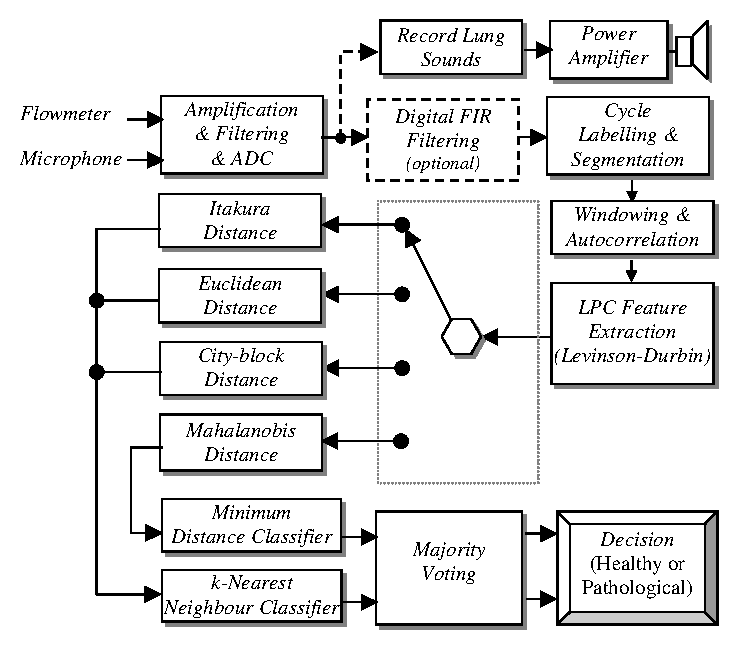
\includegraphics[scale=0.88]{figure1.eps}}
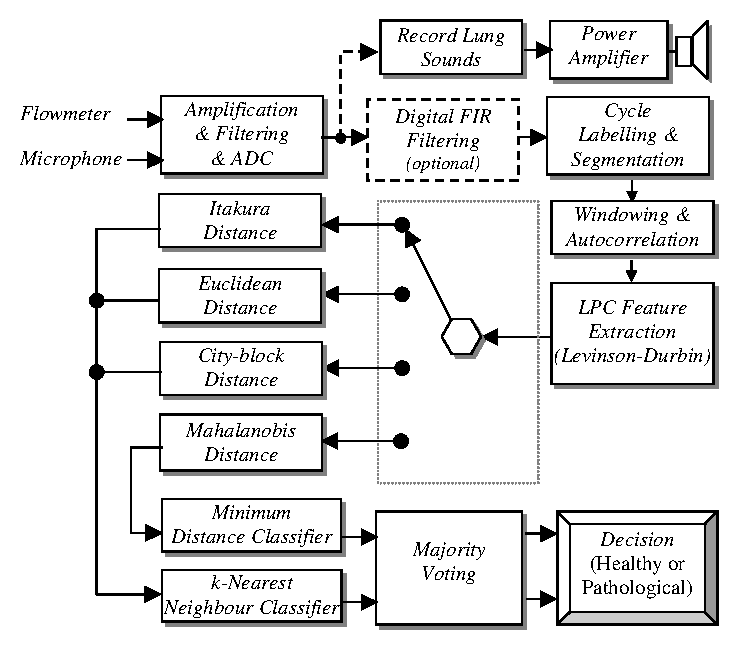
\includegraphics[scale=0.88]{figure1.eps}
\caption{Functional block diagram of the instrument.}
\label{figure1}
 \end{center}
\end{figure}



%%%%%%%%%%%%%%%%%%%%%%%%%
% SECTION START
%%%%%%%%%%%%%%%%%%%%%%%%%
\section{Background: Pulmonary sounds}
Pulmonary sounds are presumed to be produced due to air turbulence in the airways of the lungs although the exact mechanism of sound generation is still unknown. Since the lungs and the chest wall effectively act as a low-pass filter, the sounds transmitted to the skin are actually considered to be the filtered version of the original generated sounds (Sovij�rvi \etal 2000a). On the other hand, the changes in lung structure that occur in some pathological conditions change the spectrum of sounds heard over the chest wall and may further cause abnormal sounds to be auscultated. Normal lung sounds are the respiratory sounds of healthy subjects heard over the chest wall above a certain flow rate and have a frequency range of 200-600 Hz (figure~2). Pathological lung sounds, on the other hand, usually contain higher frequency components with additional respiratory sounds superimposed over them. These additional sounds are called adventitious breath sounds and, depending on their duration, they can be either continuous ({\it wheezing} if high pitched, {\it rhonchi} if low pitched), or discontinuous ({\it fine crackles} if high pitched, {\it coarse crackles} if low pitched) (Gavriely and Cugell 1995). Examples of healthy and pathological lung sounds recorded from different subjects are provided as sound files in the associated multimedia enhancements page.


%%%%%%%%%%%%%%%%%%%%%%%%%
% FIGURE START
%%%%%%%%%%%%%%%%%%%%%%%%%
\begin{figure}[t]
\begin{center}
% Uncomment the following instruction in order to
% produce a boxed version of this figure. If
% uncommented, the instruction on the following line,
% '\includegraphics[...]{...}', should be deleted.
%\fbox{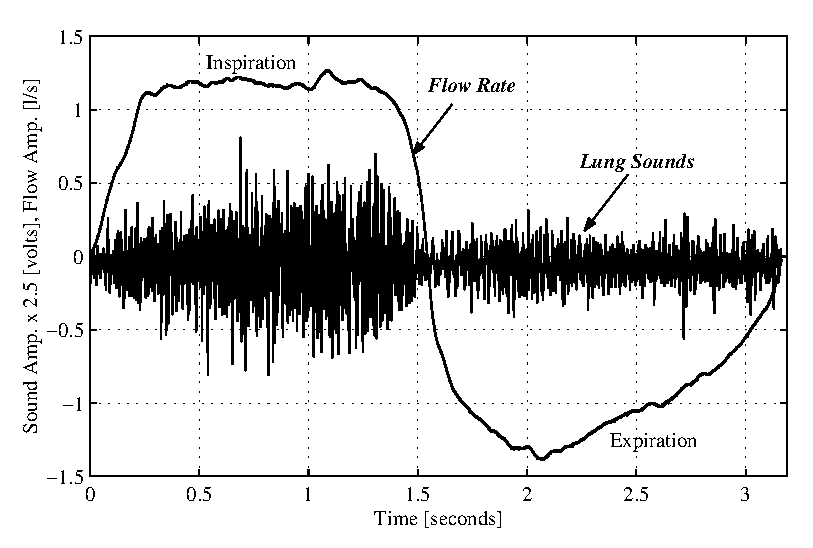
\includegraphics[width=0.67\textwidth, height=!]{figure2.eps}}
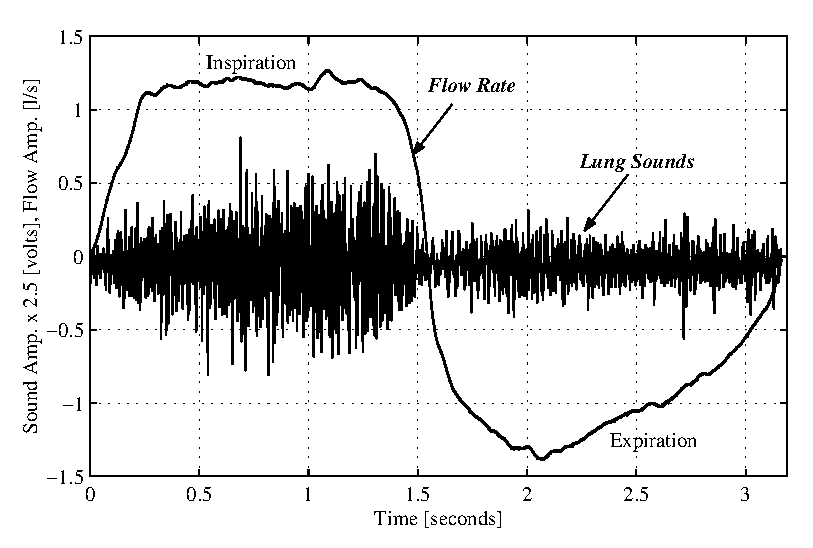
\includegraphics[width=0.67\textwidth, height=!]{figure2.eps}
\caption{Lung sound waveform and the superimposed flow rate signal of a healthy subject.}
\label{figure2}
 \end{center}
\end{figure}


Crackles, which are discontinuous and explosive adventitious lung sounds, are thought to be generated by the sudden reopening of the small airways, previously held closed by surface forces (Pasterkamp \etal 1997, Sovij�rvi \etal 2000a). Their pitch (coarse or fine), duration, number and time of occurrence bear important diagnostic information. For example, the presence or absence of crackles is used to distinguish pulmonary fibrosis from sarcoidosis; fine, late inspiratory crackles to indicate fibrotic lung disease and early, course crackles to indicate obstructive lung disease (Pasterkamp \etal 1997). Wheezes are pseudoperiodic adventitious lung sounds having a musical character and are easily detected by a stethoscope. The pathophysiologic mechanisms that are responsible of generating wheezing sounds are still not entirely clear. According to a new model, however, these sounds are presumed to be produced due to the oscillations of the airways, which occur when the airflow velocity reaches a critical value called flutter velocity due to flow limitation (Pasterkamp \etal 1997, Sovij�rvi \etal 2000a).

%%%%%%%%%%%%%%%%%%%%%%%%%
% SECTION START
%%%%%%%%%%%%%%%%%%%%%%%%%
\section{System description}
The design of the instrument is based on three interconnected functional units: the analogue processing unit, the digital processing unit and the output interface unit. A simplified block diagram of the system hardware is given in figure~3.


%%%%%%%%%%%%%%%%%%%%%%%%%
% FIGURE START
%%%%%%%%%%%%%%%%%%%%%%%%%
\begin{figure}[t]
\begin{center}
% Uncomment the following instruction in order to
% produce a boxed version of this figure. If
% uncommented, the instruction on the following line,
% '\includegraphics{...}', should be deleted.
%\fbox{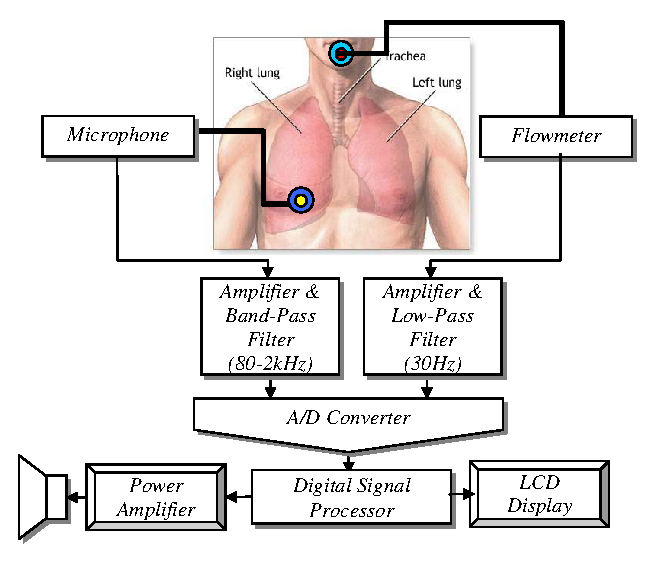
\includegraphics{figure3.eps}}
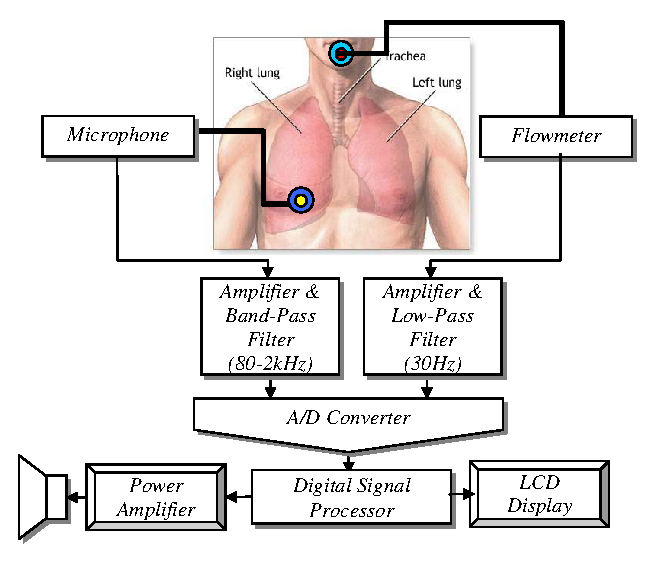
\includegraphics{figure3.eps}
\caption{A simplified block diagram of the system hardware.}
\label{figure3}
 \end{center}
\end{figure}


%%%%%%%%%%%%%%%%%%%%%%%%%
% SUBSECTION START
%%%%%%%%%%%%%%%%%%%%%%%%%
\subsection{Analogue processing unit}
The analogue processing consists of the amplification and filtering functions for the two inputs, the first of which is from a microphone attached to the posterior base of the right or left lung while the other is from a flowmeter that is used to label the lung sounds as belonging to the inspiration or expiration phase. Air-coupled electret microphones are used as pulmonary sound sensors and the geometry of the air cavity, as depicted in figure~4, is suggested by Kraman \etal (1995). The signal produced by the microphone is passed through a low noise preamplifier custom designed with low noise BJT transistors and a band-pass filter having a flat frequency response in the range 80-2000 Hz. The band-pass filter is realized by cascading a fourth order Bessel high-pass filter with an eighth order Butterworth low-pass filter. The high-pass filter is used in order to reduce the effect of the low-frequency noise resulting from cardiovascular sounds, muscles and even from the patient or microphone motion (Vannuccini \etal 2000). The Bessel filter is used in the high-pass filter configuration in order to obtain an approximately linear phase response so that waveforms containing crackles or other transients will be minimally affected. The low-pass filter is provided to eliminate the aliasing in the digitization with a sampling frequency of 8 kHz. The overall gain of the preamplifier and band-pass filter is approximately 50 dB. The response of the pulmonary sound amplifier and filter is depicted in figure~5. Simultaneously with the lung sounds, the flow signal is recorded using a Fleisch type flowmeter (CD379, Validyne Engineering) whose output is filtered with a second order Butterworth low-pass filter having a cut-off frequency at 30 Hz and then amplified using a phase-inverting amplifier having a gain of about 12 dB.


%%%%%%%%%%%%%%%%%%%%%%%%%
% FIGURE START
%%%%%%%%%%%%%%%%%%%%%%%%%
\begin{figure}[t]
\begin{center}
% Uncomment the following instruction in order to
% produce a boxed version of this figure. If
% uncommented, the instruction on the following line,
% '\includegraphics{...}', should be deleted.
%\fbox{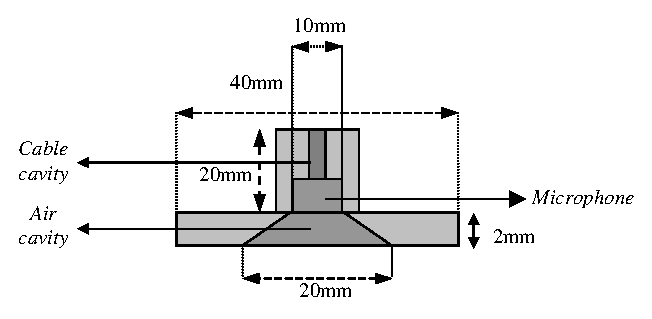
\includegraphics{figure4.eps}}
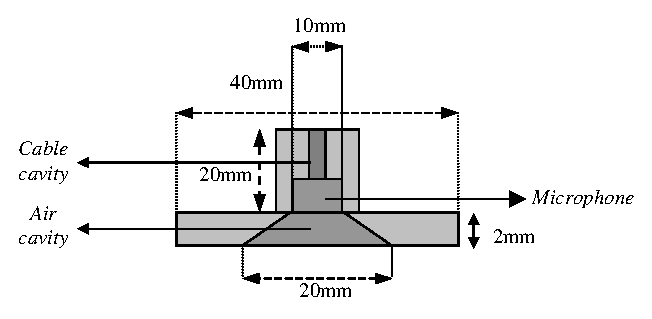
\includegraphics{figure4.eps}
\caption{Side view of the microphone capsule.}
\label{figure4}
 \end{center}
\end{figure}


%%%%%%%%%%%%%%%%%%%%%%%%%
% FIGURE START
%%%%%%%%%%%%%%%%%%%%%%%%%
\begin{figure}[t]
\begin{center}
% Uncomment the following instruction in order to
% produce a boxed version of this figure. If
% uncommented, the instruction on the following line,
% '\includegraphics[...]{...}', should be deleted.
%\fbox{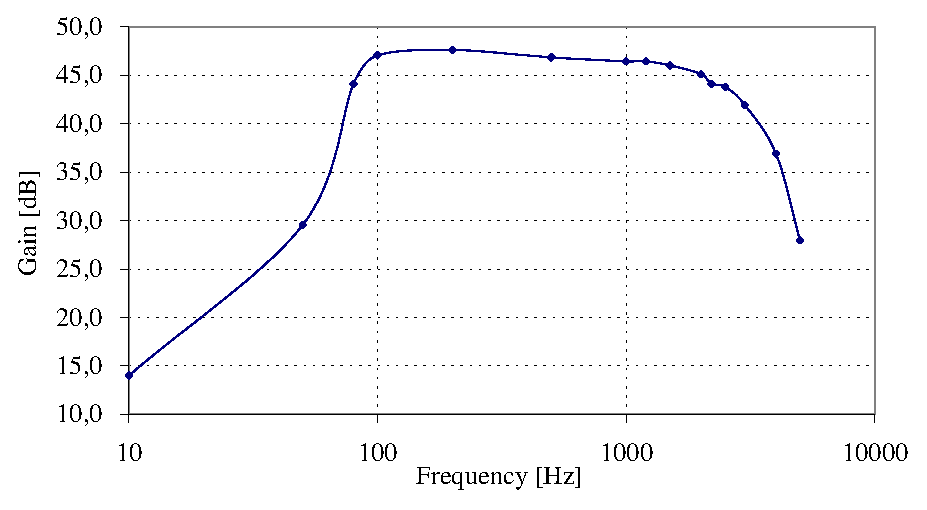
\includegraphics[scale=0.7]{figure5.eps}}
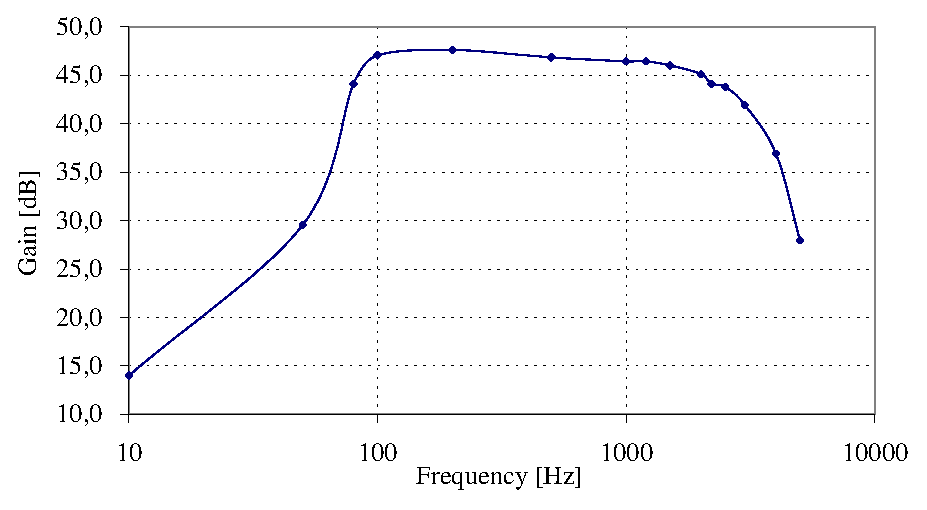
\includegraphics[scale=0.7]{figure5.eps}
\caption{The gain response of the amplifier-filter unit for the lung sounds.}
\label{figure5}
 \end{center}
\end{figure}


%%%%%%%%%%%%%%%%%%%%%%%%%
% SUBSECTION START
%%%%%%%%%%%%%%%%%%%%%%%%%
\subsection{DSP unit}
After analogue processing, both signals are digitized and processed using the DSP56311 evaluation module (EVM) manufactured by Motorola, Inc. This board includes the DSP56311 24-bit digital signal processor, 64K$\times$24-bit fast static RAM (FSRAM) for expansion memory, 128K$\times$8-bit flash memory for stand-alone operation, 16-bit audio codec and command converter circuitry (Motorola 1999a). Both of the input channels are digitized at a sampling frequency of 8 kHz using the 16-bit stereo codec integrated with the DSP56311 EVM, but the sampling rate of flow signal is reduced to 125 Hz by down sampling in 1/64 ratio. The codec (CS4218, Crystal Semiconductor) contains two delta-sigma analogue-to-digital converters, two delta-sigma digital-to-analogue converters, input anti-aliasing filters, and output smoothing filters on-chip. The codec also contains programmable output attenuators (adjustable from 0 to -46.5 in 1.5 dB steps), which were used to prevent any saturation that may result while amplifying the lung sounds with the power amplifier that feeds the external speakers.

%%%%%%%%%%%%%%%%%%%%%%%%%
% SUBSUBSECTION START
%%%%%%%%%%%%%%%%%%%%%%%%%
\subsubsection{Selecting the desired menu item.}
Three push-buttons, located on the front panel of the instrument and connected to the interrupt lines of the DSP, are used to select the desired function to be performed by the device (figure~6). The `{\it Menu}' push-button is used to call a service subroutine by which the user can navigate through all the menu items. There are a total of eight menu items available with the instrument. These items provide the user with the choices of selecting the desired classifier type and the distance measure to be used in the diagnosis process along with the options of recording, listening and digital filtering of the respiratory data. Each time the Menu push-button is pressed, a new item is displayed on the LCD. The function displayed on the LCD is executed when a second front panel push-button labelled `{\it Select}' is pressed.


%%%%%%%% SUBFIGURES %%%%%%%%%%
%%%%%%%%%%%%%%%%%%%%%%%%%
% FIGURE START
%%%%%%%%%%%%%%%%%%%%%%%%%
\begin{figure}[t]
  \centering
  \subfigure[]{
     \label{figure(a)}	%% label for first subfigure
     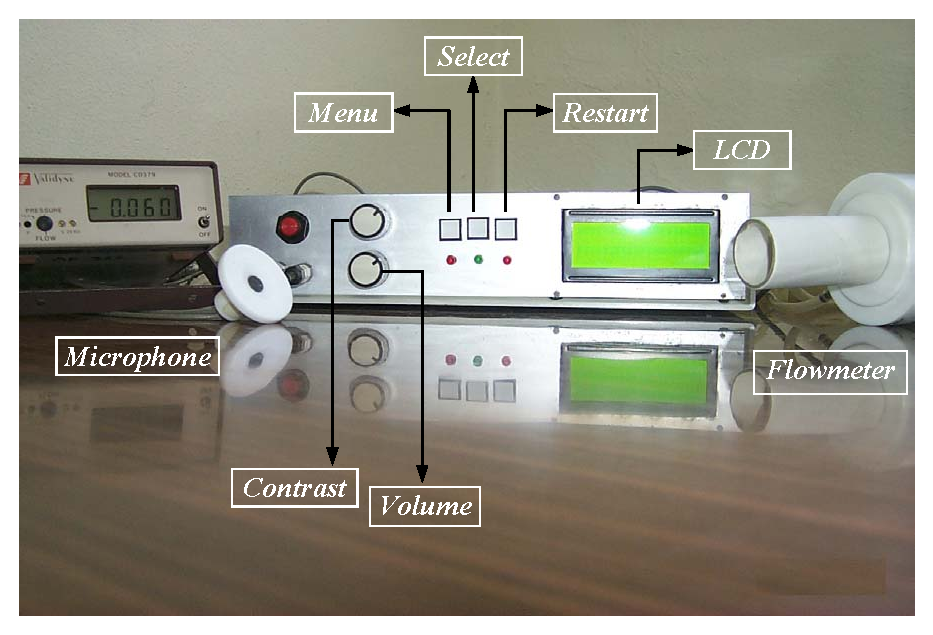
\includegraphics[width=0.47\textwidth, height=!]{figure6(a).eps}
     }
  \subfigure[]{
     \label{figure(b)}	%% label for second subfigure
     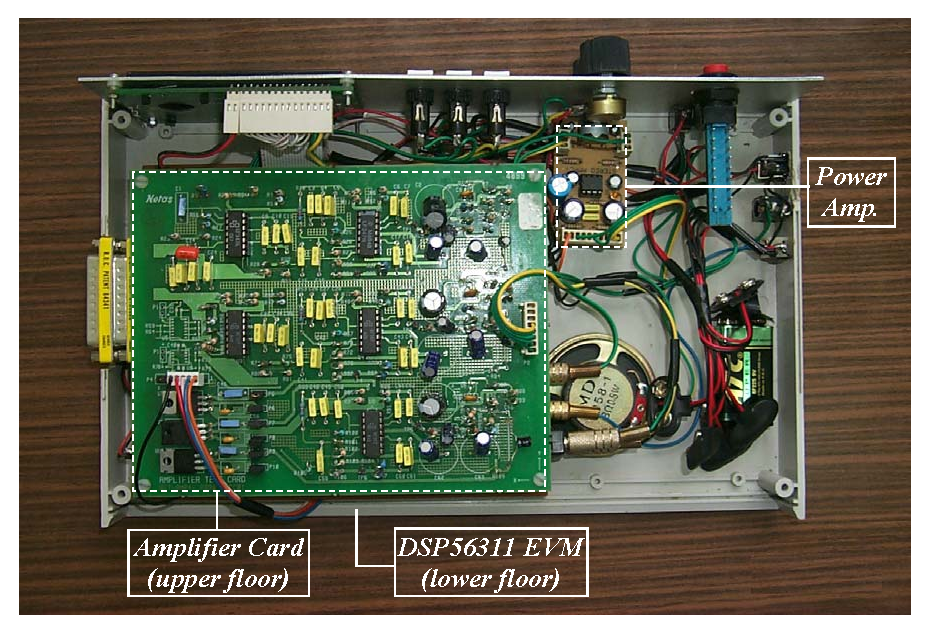
\includegraphics[width=0.47\textwidth, height=!]{figure6(b).eps}
     }
\caption{(a) The front panel of the designed pulmonary sound classification system and its (b) internal structure.}
\label{figure6}	%% label for entire figure
\end{figure}


When the classification algorithm is finished and the diagnosis result is displayed on the LCD, the DSP enters the 'Stop Processing State', the lowest power consumption mode in which all the activity of the DSP is halted. A third push-button, connected to one of the DSP's interrupt pins and labelled `{\it Restart}', is used to exit this mode and start a new test.

%%%%%%%%%%%%%%%%%%%%%%%%%
% SUBSUBSECTION START
%%%%%%%%%%%%%%%%%%%%%%%%%
\subsubsection{Recording the lung sounds.}
As stated previously, the instrument provides the user with the option of recording the sampled lung sounds for a total duration of 16 seconds to the external FSRAM found on the DSP56311 EVM. By choosing the appropriate menu item, the user may listen to the recorded lung sounds through a speaker added to the instrument. He may also listen to the lung sounds in real time as they are being sampled by using headphones.

%%%%%%%%%%%%%%%%%%%%%%%%%
% SUBSUBSECTION START
%%%%%%%%%%%%%%%%%%%%%%%%%
\subsubsection{Finite Impulse Response (FIR) filtering.}
Digital FIR filtering capability was added to this instrument. The designed filters can be applied or removed as needed by simply pressing the appropriate push-buttons. FIR filtering type was used due to the fact that these filters are guaranteed to be stable and can always be designed to have a linear phase response (El-Sharkawy 1990). This property is important in applications in which the signal shape and relative timing must be preserved. Any non-linear phase introduced by the filter may be damaging to breath sounds containing transient signals such as crackles (Vannuccini \etal 2000).

The general-purpose and fully programmable Enhanced Filter Coprocessor (EFCOP) module found on the DSP was used to do the FIR filtering process. Two digital FIR filters were designed. The first one is a band-pass FIR filter having a flat frequency response in the range 80-2000 Hz used to filter the lung sounds (figure~7). The second is a FIR low-pass filter with a cut-off frequency of 50 Hz used to filter the flow signal. For this reason, the EFCOP was operated in multichannel mode that enables the processing of multiple, equal-length channels simultaneously.


%%%%%%%%%%%%%%%%%%%%%%%%%
% FIGURE START
%%%%%%%%%%%%%%%%%%%%%%%%%
\begin{figure}[t]
\begin{center}
% Uncomment the following instruction in order to
% produce a boxed version of this figure. If
% uncommented, the instruction on the following line,
% '\includegraphics[...]{...}', should be deleted.
%\fbox{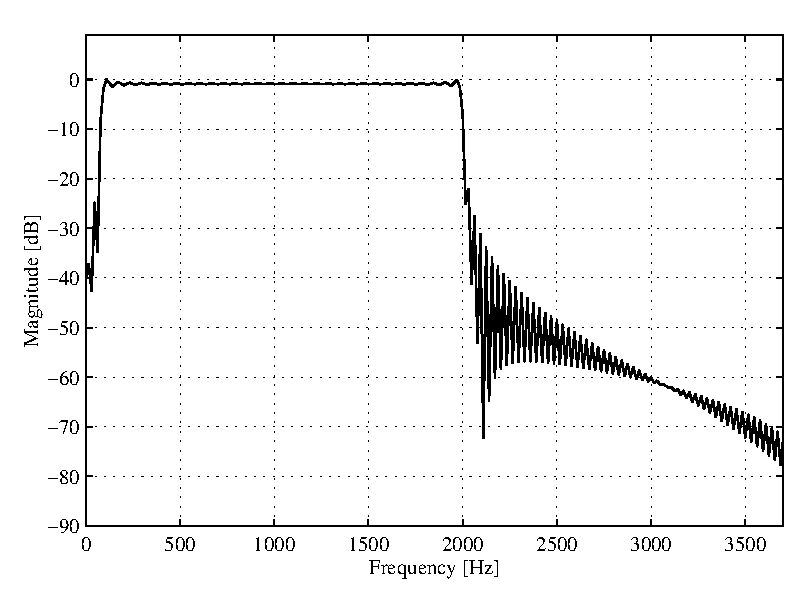
\includegraphics[width=0.67\textwidth, height=!]{figure7.eps}}
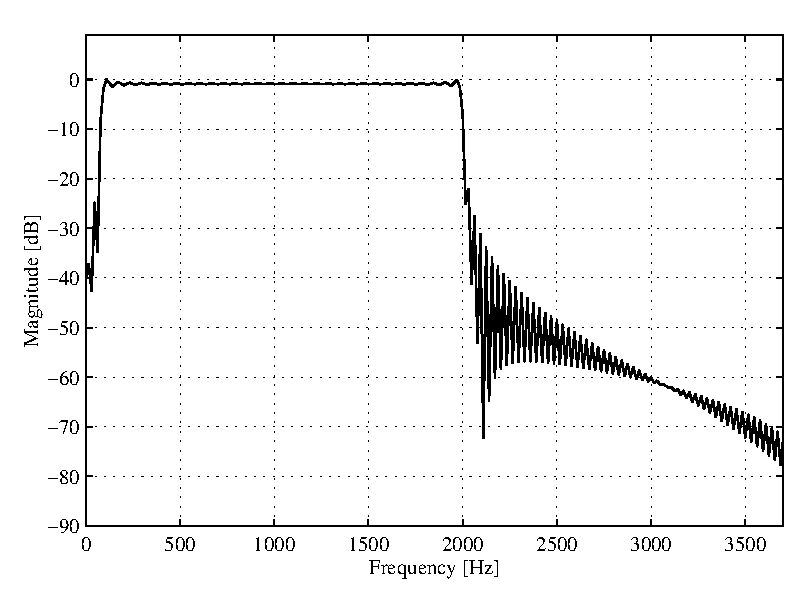
\includegraphics[width=0.67\textwidth, height=!]{figure7.eps}
\caption{The magnitude response of the FIR band-pass filter (80-2000 Hz), that can be applied on the lung sounds.}
\label{figure7}
 \end{center}
\end{figure}


%%%%%%%%%%%%%%%%%%%%%%%%%
% SUBSECTION START
%%%%%%%%%%%%%%%%%%%%%%%%%
\subsection{Output interface unit}
Communication with the outside world is achieved mainly through a liquid crystal display unit. Auxiliary interfacing options include speaker units and headphones.

%%%%%%%%%%%%%%%%%%%%%%%%%
% SUBSUBSECTION START
%%%%%%%%%%%%%%%%%%%%%%%%%
\subsubsection{Displaying messages on the LCD.}
A liquid crystal display (LCD) module (GDM2004D, Xiamen Ocular) was used for displaying the menu options, diagnosis result and other messages that convey information regarding the current state of the system. In this instrument, the most common standard used in the vast majority of LCDs, which is referred to as HD44780U (Hitachi 1999), is utilized with 8-bit mode for each ASCII character to be displayed. The control and data lines of the LCD, used for the initialization routine of the LCD module through which the interface length for communicating with the LCD, the behaviour of the cursor and its position on the screen are set, were connected to the Host Interface of the DSP, which provides a total of 16 individual pins that are fully programmable by the user.

%%%%%%%%%%%%%%%%%%%%%%%%%
% SUBSUBSECTION START
%%%%%%%%%%%%%%%%%%%%%%%%%
\subsubsection{Listening to lung sounds.}
A stereo audio amplifier was used in the output stage of the instrument to bring the output signal of the 56311EVM up to a suitable level to drive the speaker so as to listen to recorded lung sounds. This module is based on the dual audio amplifier TDA2822M (ST Microelectronics), delivering up to 5 Watt per channel into an 8 W speaker. Headphones are also provided for monitoring lung sounds as they are being sampled.

%%%%%%%%%%%%%%%%%%%%%%%%%
% SECTION START
%%%%%%%%%%%%%%%%%%%%%%%%%
\section{Autoregressive modelling of respiratory sounds}
In order to estimate the source and transmission characteristics of lung sounds, Iyer \etal (1989) investigated the application of autoregressive (AR) modelling to the analysis of these sounds. According to their model, the source of the lung sounds generated in the airways is regarded as a white noise that is produced by an additive combination of one or more of different kinds of noise sequences, thus resulting in a complete description of the lung sound sources (figure~8). Next, these sounds are considered to be the input of an all-pole filter that models the transmission of these sounds through the parenchyma and chest wall. It is also assumed that additive Gaussian noise, resulting from the instrumentation, muscle and skin, are added to these sounds during their transmission to the chest wall. Using a similar model, Hadjileontiadis and Panas (1997) investigated the use of higher-order statistics in the AR modelling of lung sounds and found that by this way the source and transmission characteristics of lung sounds were estimated efficiently, even in the presence of additive symmetric noise.


%%%%%%%%%%%%%%%%%%%%%%%%%
% FIGURE START
%%%%%%%%%%%%%%%%%%%%%%%%%
\begin{figure}[t]
\begin{center}
% Uncomment the following instruction in order to
% produce a boxed version of this figure. If
% uncommented, the instruction on the following line,
% '\includegraphics[...]{...}', should be deleted.
%\fbox{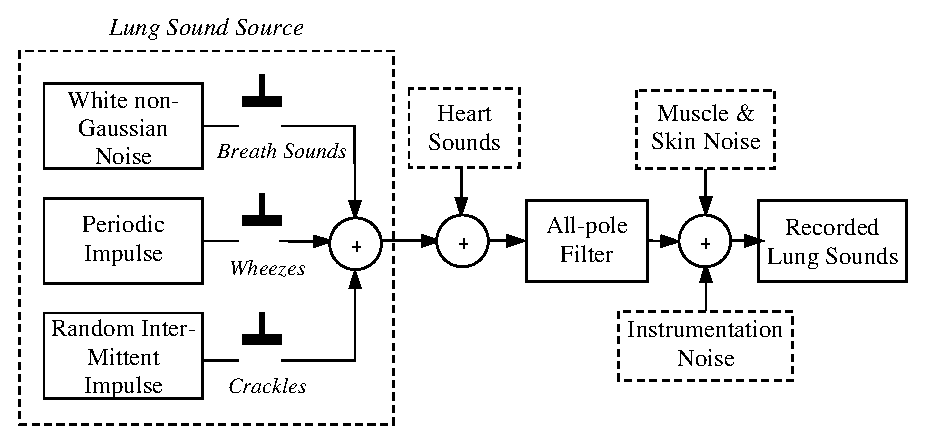
\includegraphics[scale=0.7]{figure8.eps}}
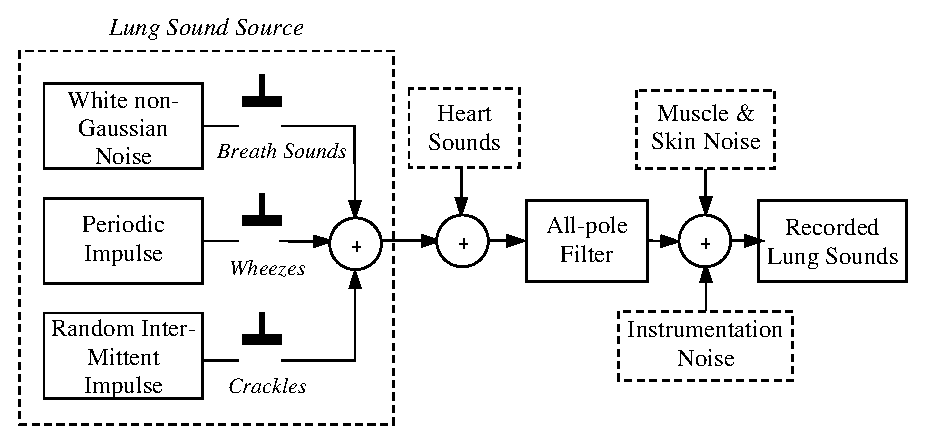
\includegraphics[scale=0.7]{figure8.eps}
\caption{All-pole modelling of lung sounds (Iyer \etal 1989).}
\label{figure8}
 \end{center}
\end{figure}


Autoregression is a modelling technique in which a weighted sum of the $p$ previous samples are used to predict the current value of the random process. This process can be described by the following equation:

%%%%%%%%%%%%%%%%%%%%%%%%%
% EQUATION START
%%%%%%%%%%%%%%%%%%%%%%%%%
\begin{equation}
\label{eqn_1}
s(n)=\sum\limits_{k =1}^p{a_k s(n-k)}+Gu(n),
\end{equation}
where $p$ is the model order, the coefficients $a_1, a_2,..., a_p$ are the prediction coefficients used to predict the next input sample, $u(n)$ is a normalized excitation and $G$ is its gain. By taking the z-transform of equation \eref{eqn_1}, the transfer function of this filter in terms of the prediction coefficients $a_k$ becomes in the form of an all-pole filter:

%%%%%%%%%%%%%%%%%%%%%%%%%
% EQUATION START
%%%%%%%%%%%%%%%%%%%%%%%%%
\begin{equation}
\label{eqn_2}
H(z)=\frac{{S(z)}}{{GU(z)}}=\frac{1}{{1 - \sum\limits_{i=1}^p{a_i z^{ - i} } }}=\frac{1}{{A(z)}}.
\end{equation}

So, the problem of linear prediction becomes determining the coefficients $a_k$ that minimize the mean-squared prediction error, thus resulting in an all-pole filter that has spectral characteristics similar to those of the analysed signal. The autocorrelation method is one of the standard methods that are typically used when all-pole modelling a signal over a finite interval (Rabiner and Juang 1993). According to this method, a data window is applied to $s(n)$, thus ensuring that the signal is set to zero outside the desired interval. This method was preferred here because it generates an all-pole model that is guaranteed to be stable. Using the property $r_x($-$k)=r_x(k)$, where $r_x(k)$ is the autocorrelation function, this method results in the following normal equations:

%%%%%%%%%%%%%%%%%%%%%%%%%
% EQUATION START
%%%%%%%%%%%%%%%%%%%%%%%%%
\begin{equation}
\label{eqn_3}
\sum\limits_{k=1}^p{r_x\left({\left|{i-k}\right|}
\right)\mathord{\buildrel{\lower3pt\hbox{$\scriptscriptstyle\frown$}}
\over a}_k=r_x (i)}.
\end{equation}

The set of equations in the form of equation \eref{eqn_3}, are known as the Yule-Walker equations and they arise often in minimum mean square problems (Hayes 1996, Rabiner and Juang 1993). These equations can be represented in the matrix form $\bi{R}\bi{a}=\bi{r}$. Fortunately, the Toeplitz structure (equal values along each diagonal) of the autocorrelation matrix $\bi{R}$ leads to normal equations that can be solved using iterative and efficient methods such as the Levinson-Durbin algorithm.

The Levinson-Durbin algorithm was implemented on the DSP56311, which is a fixed-point processor that uses fractional data representation for all of its arithmetic operations. Since DSP56311 is a 24-bit machine, the word values that can be represented will be limited by the most negative and most positive numbers $-1.0$ and $1-2^{-23}=0.9999998$, respectively (Chrysafis and Lansdowne 1988). However, the Levinson-Durbin algorithm is considered to be recursive in the model order and the calculated AR coefficients are not guaranteed to be in the range $[-1,+1)$. As a result, the algorithm was modified so as to include appropriate scaling to prevent overflow (Grassi 1998).

Segments consisting of Hamming windowed real data samples were used in computing AR parameters. The model order used in this work was chosen as 6 (Vanderschoot \etal 1992). As will be explained in the next section, for any of the classifiers selected by the user, each respiratory cycle, divided into 60 frames, requires the calculation of $6\times60$ autocorrelation coefficients followed by the calculation of another 6x60 AR coefficients. Then, these coefficients are stored sequentially in DSP's memory to be used in the classification process. Finally, after classifying all of the 60 feature vectors individually, with 10 vectors in each subphase feature space separately, a simple majority voting algorithm is used to classify the whole stored respiratory cycle.

%%%%%%%%%%%%%%%%%%%%%%%%%
% SECTION START
%%%%%%%%%%%%%%%%%%%%%%%%%
\section{The classification algorithms}
By pressing the Menu push-button located on the front panel of the instrument, the user may choose to perform the classification process using either a $k$-NN (with $k=5$) based classifier or a minimum distance based classifier (Cohen 1986). The instrument provides the user with the option of choosing different distance measures with the k-NN classifier. These are the Itakura, Euclidean and city-block distance measures. The minimum distance classifier, on the other hand, is based on the Mahalanobis distance measure.

%%%%%%%%%%%%%%%%%%%%%%%%%
% SUBSECTION START
%%%%%%%%%%%%%%%%%%%%%%%%%
\subsection{The storage and segmentation of respiratory data}
A single respiratory cycle is needed for each subject and only data that correspond to flow rates above a threshold of 10\% of the maximum flow signal value are used for the classification process. Therefore, whenever the user selects one of the classifiers, the instrument starts to wait for the patient to start breathing through the flowmeter. As soon as this cycle is detected, the system starts storing the respiratory sounds and the corresponding flow signal. To prevent the storage of false cycles resulting from noise or even from the nature of the flow signal itself, inspiration or expiration phases lasting shorter than 0.6 second are ignored ($<$ 5000 samples).

The status of the recording process is reflected in real-time to the user using three light-emitting diodes (LEDs) located on the front panel of the instrument. The first and second LEDs indicate that the breath sounds belonging to the inspiration and expiration phases are being stored, respectively. The third LED, on the other hand, blinks whenever the storage process has ended, thus informing the patient that he can stop breathing through the flowmeter. These LEDs are connected to the output pins of the timers found in the DSP56311 internal triple timer module.

The stored respiratory cycle is divided into six distinctive subphases according to the information they bear and the different mechanisms that generate them: early, mid, late inspiratory, and early, mid, late expiratory subphases. Each respiratory subphase is further divided into ten 25\% overlapping segments. The start and end addresses of these subphases are determined according to the airflow volume calculated by integrating the stored inspiratory and expiratory flow samples separately. The early, mid and late inspiration/expiration subphases correspond to intervals contributing to the first 30\%, next 40\% and the last 30\% of the total inspiration/expiration air flow volume, respectively. As a result of segmentation of the stored full respiratory cycle, there is a total of 60 segments from which AR coefficients are extracted and used in the classification process (figure~9).


%%%%%%%%%%%%%%%%%%%%%%%%%
% FIGURE START
%%%%%%%%%%%%%%%%%%%%%%%%%
\begin{figure}[t]
\begin{center}
% Uncomment the following instruction in order to
% produce a boxed version of this figure. If
% uncommented, the instruction on the following line,
% '\includegraphics[...]{...}', should be deleted.
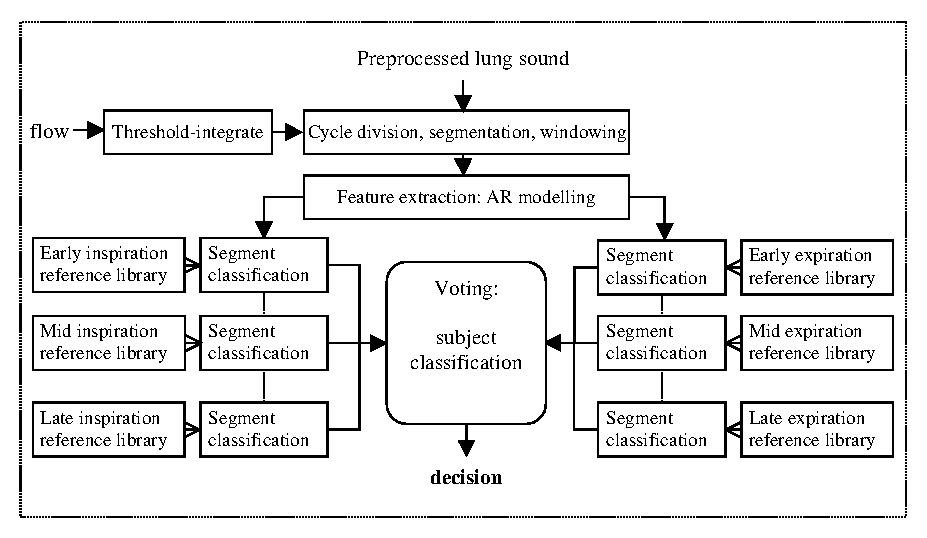
\includegraphics[scale=0.8]{figure9.eps}
\caption{Block diagram of the classification algorithm.}
\label{figure9}
 \end{center}
\end{figure}


%%%%%%%%%%%%%%%%%%%%%%%%%
% SUBSECTION START
%%%%%%%%%%%%%%%%%%%%%%%%%
\subsection{Classification with k-NN classifier}
The k-NN classifier is a nonparametric decision procedure in which the segment under test is classified by examining the categories of the nearest {\it k} neighbours and taking a majority vote (Cohen 1986, Duda and Hart 1973). In this work, the k-NN classifier was implemented using three different distance metrics: Itakura, Euclidean, and city-block distance measures. Itakura distance measure is a popular metric used in the case of AR modelling. This metric is defined as the logarithmic ratio of the minimum total squared predictor errors of the reference and test patterns. If the AR coefficients of the {\it lth} reference pattern of the {\it ith} class (the healthy or the pathological class), and the {\it mth} test pattern are denoted as $\bi{b}_{i,l}$ and $\bi{a}_m$, respectively, and $\bi{R}$ is the autocorrelation matrix of the observation vector, then this distance can be written as (Allerhand 1987) :

%%%%%%%%%%%%%%%%%%%%%%%%%
% EQUATION START
%%%%%%%%%%%%%%%%%%%%%%%%%
\begin{equation}
\label{eqn_4}
d_{m,l}=\log _{10}\frac{{\bi{b}_{i,l}^T \bi{R}\bi{b}_{i,l}}}{{\bi{a}_m^T\bi{R}\bi{a}_m}}.
\end{equation}

The Euclidean distance measure, on the other hand, is defined according to the equation:

%%%%%%%%%%%%%%%%%%%%%%%%%
% EQUATION START
%%%%%%%%%%%%%%%%%%%%%%%%%
\begin{equation}
\label{eqn_5}
d_{m,l}=\left[{(\bi{a}_m -\bi{b}_{i,l})^T(\bi{a}_m-\bi{b}_{i,l})}\right]^{1/2}.
\end{equation}

The last distance measure tested with the k-NN classifier is the city-block or Hamming metric, which is defined as the summation of the elements of the vector $\left| {\bi{a}_m-\bi{b}_{i,l}}\right|
$ (Allerhand 1987). When compared with the Euclidean distance measure, this metric has the advantage of not requiring any multiplication or square root calculation process, thus making its implementation on a fixed-point DSP simpler and more accurate.

%%%%%%%%%%%%%%%%%%%%%%%%%
% SUBSECTION START
%%%%%%%%%%%%%%%%%%%%%%%%%
\subsection{Classification with minimum distance classifier}
The distance measure used with the minimum distance classifier is the quadratic Mahalanobis metric, which is defined as:

%%%%%%%%%%%%%%%%%%%%%%%%%
% EQUATION START
%%%%%%%%%%%%%%%%%%%%%%%%%
\begin{equation}
\label{eqn_6}
d_{m,i}=\left({\bbeta_m^{(x)}-\bbeta_i}\right)^T\bi{W}_i^{- 1}\left({\bbeta_m^{(x)}-\bbeta_i} \right),
\end{equation}
where $\bbeta_m^{(x)}$ is the feature vector of the segment to be classified, $\bbeta_i$ is the estimated mean feature vector and $\bi{W}_i$ is the class covariance matrix belonging to class {\it i}. The modelling error of each segment is added to the AR parameters to be used as the feature vector. Thus, each feature vector consists of seven elements (6 AR parameters + modelling error).

The Mahalanobis distance differs fundamentally from the Euclidean distance in that the shape of the statistical density of the data is taken into account, so that the distance represents the number of {\it standard deviations} away from the mean. However, the covariance matrices can be hard to determine accurately although they have to be calculated only once. Nonetheless, when compared with the k-NN classifier, this distance measure has the advantage of requiring less memory because each class is represented by only 6 mean feature vectors and 6 inverse covariance matrices.

%%%%%%%%%%%%%%%%%%%%%%%%%
% SUBSECTION START
%%%%%%%%%%%%%%%%%%%%%%%%%
\subsection{Forming the reference libraries}
The subjects used for forming the feature vectors and templates representing the pathological class consisted of 21 patients having various restrictive (such as pulmonary fibrosis, pneumonia and pulmonary edema) and obstructive pulmonary diseases (such as asthma, bronchitis and emphysema). These pathological cases were confirmed by the auscultations made by physicians, by pulmonary function tests and by chest film findings. The respiratory sounds of those subjects representing the healthy class, on the other hand, consisted of 21 non-smoking male subjects whose ages were between 22 and 35. The database containing these sounds was formed by our laboratory (Lung Acoustics Lab.) using a commercial multichannel 12-bit data acquisition card (DAQ500 card, National Instruments) with a user interface written using LabVIEW (National Instruments). In these recordings, the posture used was a sitting position, and the microphones were usually attached to the right and left posterior base of the lungs (Rossi \etal 2000). However, in some cases the physician was asked to mark the regions of the lungs where the pathological sounds were most audible, and the microphones were attached to that area.

To find out the {\it dynamic range} needed for implementing the different classifiers, a similar program to the one running on the DSP was implemented in MATLAB 6.0 (MathWorks, Inc.) environment. This program was also used for forming the feature vectors (AR parameters) needed for training the k-NN based classifiers, and the templates (mean feature vectors and covariance matrices) needed for training the minimum distance classifier available with the instrument.

%%%%%%%%%%%%%%%%%%%%%%%%%
% SUBSUBSECTION START
%%%%%%%%%%%%%%%%%%%%%%%%%
\subsubsection{Reference library for the k-NN classifier.}
While forming the reference library for the k-NN classifiers, each respiratory cycle referring to each subject was divided into 60 overlapping segments in a similar way to the segmentation process done by the software running on the DSP. The AR parameters of each frame were determined using the available Levinson-Durbin function of MATLAB. This process was repeated for all the 42 subjects (21 healthy + 21 pathological). As a result, each subject was represented by (60 segments)$\times$(AR\_order+1) coefficients, where the AR order was chosen as six.

%%%%%%%%%%%%%%%%%%%%%%%%%
% SUBSUBSECTION START
%%%%%%%%%%%%%%%%%%%%%%%%%
\subsubsection{Reference library for the minimum distance classifier.}
As it is seen from equation \eref{eqn_6}, the classification based on Mahalanobis distance measure requires calculating the mean feature vectors and the inverse covariance matrices that represent the classes to be classified. The reference library consisting of these templates belonging to the healthy and pathological lung sounds corresponding to the six respiratory subphases were computed using MATLAB according to the following two equations:



%%%%%%%%%%%%%%%%%%%%%%%%%
% EQUATION START
%%%%%%%%%%%%%%%%%%%%%%%%%
\begin{equation}
\label{eqn_7}
\bbeta_i=\frac{1}{{KM}}\sum\limits_{k=1}^K{\sum\limits_{m=1}^M{\bbeta_m^{(k)}}},
\end{equation}

%%%%%%%%%%%%%%%%%%%%%%%%%
% EQUATION START
%%%%%%%%%%%%%%%%%%%%%%%%%
\begin{equation}
\label{eqn_8}
\bi{W}_i=\frac{1}{{KM}}\sum\limits_{k=1}^K{\sum\limits_{m=1}^M{(\bbeta_m^{(k)}-\bbeta_i)(\bbeta_m^{(k)}-\bbeta_i)^T}},
\end{equation}
where {\it K} is the total number of respiratory cycles in the related class, {\it M} is the total number of averaged feature vectors for one respiratory subphase. In this work, the number of subjects in each class was 21, and each respiratory subphase was divided into 10 overlapping segments. So, the values of {\it K} and {\it M} were taken as 21 and 10, respectively. Thus, in the minimum distance classifier each class requires the storage of six inverse covariance matrices and six mean feature vectors, each one corresponding to a different respiratory subphase.

%%%%%%%%%%%%%%%%%%%%%%%%%
% SECTION START
%%%%%%%%%%%%%%%%%%%%%%%%%
\section{Classification results}
To have a prior idea about the performance of the instrument before operating it in real-time in clinical environment, the performance of the different classifiers was measured offline using the leave-one-out method. According to this method, the training set of each classifier was formed from all subjects' feature vectors except the one sample to be classified. Next, the feature vectors corresponding to the subject to be classified were stored directly in the allocated memory of the DSP. This process was repeated for all the 42 subjects found in the training set.

Three parameters (sensitivity, specificity, and accuracy) were calculated for measuring the performance of all the classifiers (figure~10). Here, sensitivity is defined as the ratio of the number of pathological subjects classified correctly to the total number of pathological subjects. Specificity is the number of healthy subjects classified correctly divided by the total number of healthy subjects, while accuracy is defined as the number of subjects correctly classified divided by the total number of subjects in the training set.


%%%%%%%%%%%%%%%%%%%%%%%%%
% FIGURE START
%%%%%%%%%%%%%%%%%%%%%%%%%
\begin{figure}[t]
\begin{center}
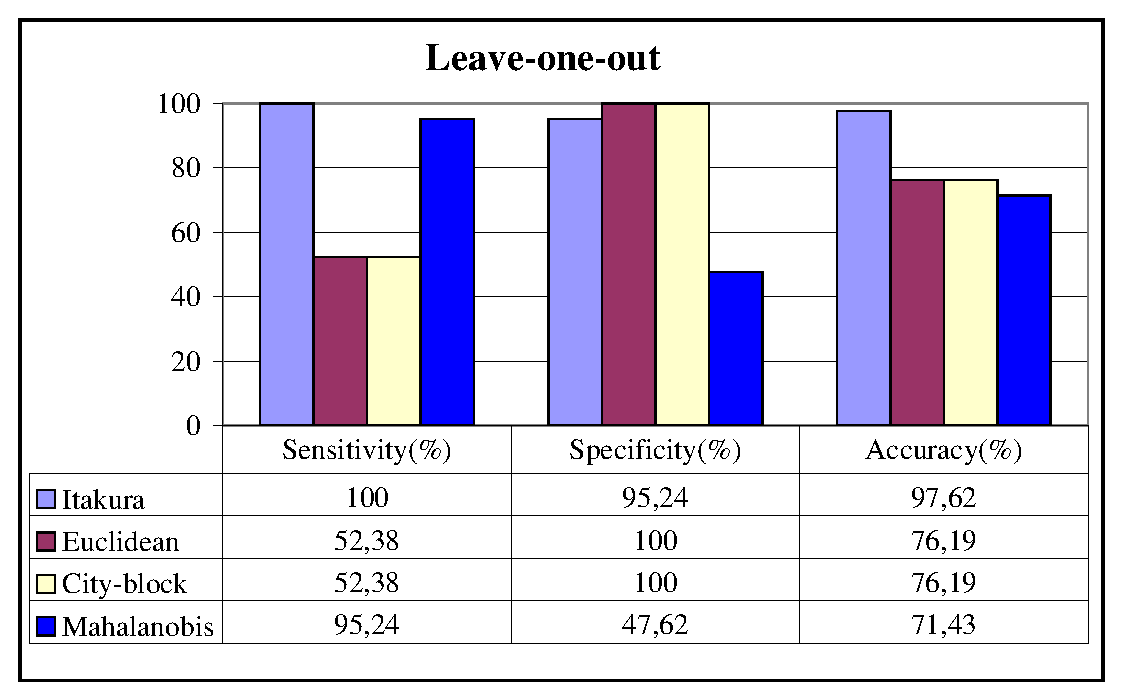
\includegraphics[scale=0.57]{figure10.eps}
\caption{Performance results of different classifiers using the leave-one-out method. K-nearest neighbour
classifier is used with Itakura, Euclidean and City-block distance measures and Minimum Distance classifier is used with Mahalanobis distance.}
\label{figure10}
\end{center}
\end{figure}




%%%%%%%%%%%%%%%%%%%%%%%%%%%%%%%%%%%%%%%%%%%%%%%%
% TABLE START
%%%%%%%%%%%%%%%%%%%%%%%%%%%%%%%%%%%%%%%%%%%%%%%%
% If desired, this table can be used instead of figure 10 by only removing the comment signs at the
% beginning of each line, and by commenting out the lines referring to figure 10 written above.
% However, in this case, the reference to this table in the text should be changed accordingly, i.e.
% reference to 'figure 10' in the text should be replaced with 'table 10'.
%%%%%%%%%%%%%%%%%%%%%%%%%%%%%%%%%%%%%%%%%%%%%%%%
%\begin{table}
%\caption{\label{table1}Performance results of different classifiers using the leave-one-out method.
%K-nearest neighbour classifier is used with Itakura, Euclidean and City-block distance
%measures and Minimum Distance classifier is used with Mahalanobis distance.}
%\begin{indented}
%\lineup
%\item[]\begin{tabular}{@{}*{7}{l}}
%\br                              
%&Sensitivity&Specificity&Accuracy\cr 
%Distance measure&(\%)&(\%)&(\%)\cr 
%\mr
%Itakura&100&\095.24&97.62\cr
%Euclidean&\052.38&100&76.19\cr
%City-block&\052.38&100&76.19\cr
%Mahalanobis&\095.24&\047.62&71.43\cr
%\br
%\end{tabular}
%\end{indented}
%\end{table}




To further investigate the performance of the instrument when operated in real time, only the more successful k-NN based classifiers were used to classify a total of 20 real subjects: 9 with pathological and 11 with healthy respiratory sounds. Those subjects with pathological sounds consisted of 4 female and 5 male patients suffering from various restrictive or/and obstructive respiratory diseases. On the other hand, a total of 11 healthy subjects (10 male+1 female) were used to test the online performance of the healthy class (figure~11).


%%%%%%%%%%%%%%%%%%%%%%%%%
% FIGURE START
%%%%%%%%%%%%%%%%%%%%%%%%%
\begin{figure}[t]
\begin{center}
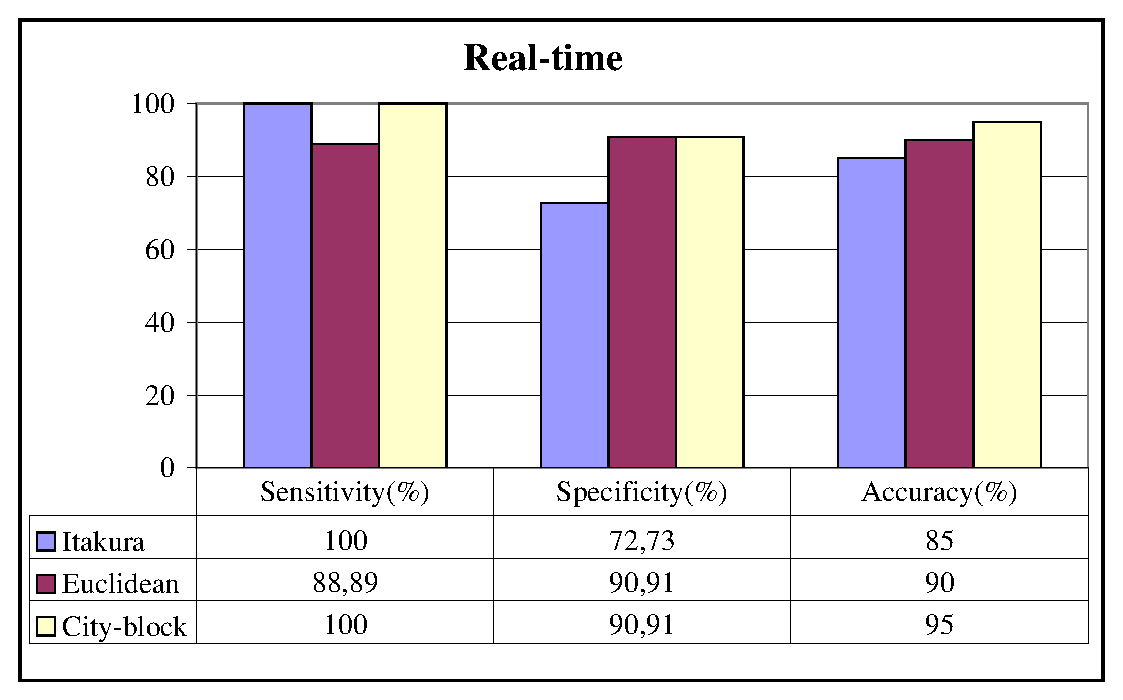
\includegraphics[scale=0.57]{figure11.eps}
\caption{Performance results of real-time classification with K-nearest neighbour classifier using different distance measures.}
\label{figure11}
\end{center}
\end{figure}





%%%%%%%%%%%%%%%%%%%%%%%%%%%%%%%%%%%%%%%%%%%%%%%%
% TABLE START
%%%%%%%%%%%%%%%%%%%%%%%%%%%%%%%%%%%%%%%%%%%%%%%%
% If desired, this table can be used instead of figure 11 by only removing the comment signs at the
% beginning of each line, and by commenting out the lines referring to figure 11 written above.
% However, in this case, the reference to this table in the text should be changed accordingly, i.e.
% reference to 'figure 11' in the text should be replaced with 'table 11'.
%%%%%%%%%%%%%%%%%%%%%%%%%%%%%%%%%%%%%%%%%%%%%%%%
%\begin{table}
%\caption{\label{table2}Performance results of real-time classification with K-nearest neighbour
%classifier using different distance measures.}
%\begin{indented}
%\lineup
%\item[]\begin{tabular}{@{}*{7}{l}}
%\br                              
%&Sensitivity&Specificity&Accuracy\cr 
%Distance measure&(\%)&(\%)&(\%)\cr
%\mr
%Itakura&100&72.73&85\cr
%Euclidean&\088.89&90.91&90\cr
%City-block&100&90.91&95\cr
%\br
%\end{tabular}
%\end{indented}
%\end{table}




In addition to the diagnosis result, the ratio of the votes of the winner class to the total number of segments classified by the DSP is also displayed on the LCD. This information is added to the diagnosis result so as to give the user an idea about the severity of the pathology. However, it should be mentioned here that the displayed number is only a measure of the similarity between the feature vectors of the lung sounds to be classified and the reference library representative of the winner class.

%%%%%%%%%%%%%%%%%%%%%%%%%
% SECTION START
%%%%%%%%%%%%%%%%%%%%%%%%%
\section{Conclusions and discussions}
The analysis of respiratory sounds in real time is considered to be important for several reasons. First of all, almost instantaneous results are obtained. Therefore, the effect of changes due to treatment, for example, may be observed and measured as they occur. In addition, any errors in the environment or the equipment can be identified immediately, thus reducing the chance of producing wrong conclusions (Sun \etal 1998). Since the analysis is made on respiratory sounds as they are being captured, this also has the advantage of reducing the storage requirements.

In this work, a DSP based instrument was designed for the classification of lung sounds as belonging to only two classes and very encouraging results were obtained. In general, it has been shown that the performance of k-NN based classifiers was much better than that of the minimum distance classifier. This result is consistent with the one obtained by Sankur \etal (1994). To be more specific, the performance measurements made using the leave-one-out method showed that k-NN based on Itakura distance measure gave the highest accuracy value among all the other distance measures. In fact, it was able to classify all the subjects except one healthy subject, thus giving an accuracy value of 97.62\%. The relatively lower accuracy value of the minimum distance classifier, however, can be explained by the fact that in this classifier each class was represented by only six averaged feature vectors and six averaged covariance matrices representing each respiratory subphase. For the pathological case, these values were obtained by averaging the feature vectors of 21 subjects having a wide variety of pulmonary diseases, with each disease having distinct characteristics. For this reason, this averaging of the feature vectors, probably, did not yield a faithful representation of this class.

The real-time performance of the instrument resulted in high accuracy values ranging between 85 to 95\%. The sensitivity results were also high ranging between 88.89 to 100\%, indicating that almost all pathological subjects were correctly identified. This performance is a promising feature of the instrument for its applicability in clinical environment. The online classification results also showed that the relatively simpler city-block distance measure showed the best accuracy value among all the k-NN classifiers although the leave-one-out performance results showed that the Euclidean and city-block distance measures gave equal but relatively lower accuracy values.

In general, the only means by which the performance of the k-NN classifier can be improved is by increasing the number of training set patterns. However, these patterns have to be stored individually, which requires large memory. Another disadvantage of the k-NN classifier is that it requires large computing power since in order to classify a segment its distance to all the segments in training set has to be calculated.

In this study, the classification of lung sounds to only two classes was investigated. The next step can be the classification into three classes: restrictive, obstructive and healthy lung sounds. However, this requires increasing the database representative of each class. The only obstacle here will be the large amount of memory and computing power that will be needed by the instrument.


%%%%%%%%%%%%%%%%%%%%%%%%%
% ACKNOWLEDGMENTS START
%%%%%%%%%%%%%%%%%%%%%%%%%
\ack
This work was supported by Bo�azi�i University Research Fund (project no 02A202). Authors would like to acknowledge and pay special thanks to Prof. Dr. G�nseli K�l�n� from Cerrahpa�a medical faculty of �stanbul University and Dr. Filiz S�ng�n from Heybeliada Sanatorium for their assistance during our visits to their hospitals.




%%%%%%%%%%%%%%%%%%%%%%%%%
% REFERENCES START
%%%%%%%%%%%%%%%%%%%%%%%%%
\References

\item[] Ackenhusen J G 1999 {\it Real-Time Signal Processing: Design and Implementation of Signal Processing Systems} (Upper Saddle River, NJ: Prentice Hall) pp~1--116

\item[] Allerhand M 1987 {\it Knowledge-Based Speech Pattern Recognition} (London: Kogan Page) pp~49--131

\item[] Chrysafis A and Lansdowne S 1988 {\it Fractional and Integer Arithmetic Using the DSP56000 Family of General-Purpose Digital Signal Processors, APR3/D} (USA: Motorola, Inc.)

\item[] Cohen A 1986 {\it Biomedical Signal Processing} vol 2 (Boca Raton, Florida: CRC Press) pp~50--60

\item[] Duda R O and Hart P E 1973 {\it Pattern Classification and Scene Analysis} (New York: John Wiley) pp~10--105

\item[] Earis J E and Cheetham B M G 2000 Current methods used for computerized respiratory sound analysis {\it Eur. Respir. Rev.} {\bf 10} 586--90

\item[] El-Sharkawy M 1990 {\it Real Time Digital Signal Processing Applications with Motorola's DSP56000 Family} (Englewood Cliffs, NJ: Prentice Hall)

\item[] Gavriely N and Cugell D W 1995 {\it Breath Sounds Methodology} (Boca Raton, Florida: CRC Press)

\item[] Grassi S 1998 Optimized implementation of speech processing algorithms {\it PhD Thesis} University of Neuch�tel, IMT, Switzerland

\item[] Hadjileontiadis L J and Panas S M 1997 Autoregressive modeling of lung sounds using higher-order statistics: estimation of source and transmission {\it IEEE Signal Processing Workshop on Higher-Order Statistics (Banff, Alberta, Canada, July 1997)} pp~4--8

\item[] Hayes M H 1996 {\it Statistical Digital Signal Processing and Modeling} (New York: John Wiley \& Sons)

\item[] Hitachi 1999 {\it HD44780U (LCD-II) Dot Matrix Liquid Crystal Display Controller/Driver, ADE-207-272(Z), Rev. 0.0} (Tokyo, Japan: Hitachi, Ltd.)

\item[] Iyer V K, Ramamoorthy A and Ploysongsang Y 1989 Autoregressive modeling of lung sounds: characterization of source and transmission {\it IEEE Trans. Biomed. Eng.} {\bf 36} 1133--7

\item[] Kraman S S, Wodicka G R, Oh Y and Pasterkamp H 1995 Measurement of respiratory acoustic signals. Effect of microphone air cavity width, shape, and venting {\it Chest} {\bf 108} 1004--8

\item[] Motorola 1999a {\it DSP56311 Evaluation Module Hardware Reference Manual, DSP56311EVMUM/D, Rev. 1.8} (USA: Motorola, Inc.)

\item[]\dash 1999b {\it DSP56311 User's Manual, DSP56311UM/D, Rev. 1.0} (USA: Motorola, Inc.)

\item[] Pasterkamp H, Kraman S S and Wodicka G R 1997 Respiratory sounds: advances beyond the stethoscope {\it Am. J. Respir. Crit. Care Med.} {\bf 156} 974--87

\item[] Petty T L, Weinmann G G 1997 Building a national strategy for the prevention and management of and research in chronic obstructive pulmonary disease. National Heart, Lung and Blood Institute Workshop Summary {\it JAMA} {\bf 277} 246--53

\item[] Rabiner L R and Juang B H 1993 {\it Fundamentals of Speech Recognition} (Englewood Cliffs, NJ: Prentice Hall)

\item[] Rossi M, Sovij�rvi A R A, Piiril� P, Vannuccini L, Dalmasso F and Vanderschoot J 2000 Environmental and subject conditions and breathing manoeuvres for respiratory sound recordings {\it Eur. Respir. Rev.} {\bf 10} 611--5.

\item[] Sankur B, Kahya Y P, G�ler E � and Engin T 1994 Comparison of AR based algorithms for respiratory sound classification {\it Comput. Biol. Med.} {\bf 21} 67--76

\item[] Smyllie H C, Blendis L M and Armitage P 1965 Observer disagreement in physical signs of the respiratory system {\it Lancet} {\bf 2} 412--4

\item[] Sovij�rvi A R A, Malmberg L P, Charbonneau G, Vanderschoot J, Dalmasso F, Sacco C, Rossi M and Earis J E 2000a Characteristics of breath sounds and adventitious respiratory sounds {\it Eur. Respir. Rev.} {\bf 10} 591--6

\item[] Sovij�rvi A R A, Vanderschoot J and Earis J E 2000b Standardization of computerized respiratory sound analysis {\it Eur. Respir. Rev.} {\bf 10} 585

\item[] Sun X, Cheetham B M G and Earis J E 1998 Real time analysis of lung sounds {\it Technol. Health Care} {\bf 6} 3--10

\item[] Vanderschoot J, Coppello N G J and Schreur H J W 1992 AR model orders of lung sounds {\it Proc. Ann. Int. Conf. IEEE Eng. Med. Biol. Soc.} vol 14 pp~2531--2

\item[] Vannuccini L, Earis J E, Helist� P, Cheetham B M G, Rossi M, Sovij�rvi A R A and Vanderschoot J 2000 Capturing and preprocessing of respiratory sounds {\it Eur. Respir. Rev.} {\bf 10} 616--20


\endrefs




\end{document}

